\section{Package Model}\begin{figure}[h!]
\begin{center}
	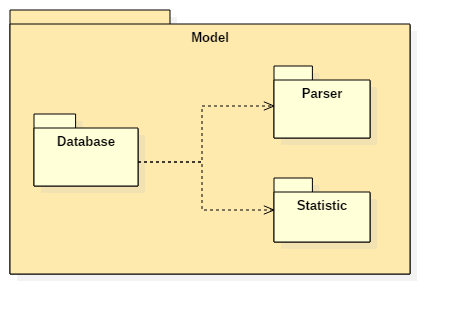
\includegraphics[scale=0.7]{../images/ModelPackage.png}
\end{center}
\end{figure}
\subsection{Model::Database}
\subsubsection{Model::Database::UserManager}
\begin{itemize}
\item\textbf{Funzione del componente:} la classe permettera' l'inserimento, la lettura e la rimozione di utenti all'interno della collezione
			\item\textbf{Relazioni d'uso con altre componenti:} interagisce con la ViewModel, gestendone le richieste di interazione sugli utenti\\ \\
La classe utilizza:
	\begin{itemize}
		\item
	\end{itemize}
\item\textbf{Attributi}:
	\begin{itemize}
		\item\code{}\\
		\item\code{}\\
		\item\code{}\\
		\item\code{}\\
	\end{itemize}
\item\textbf{Metodi}:
	\begin{itemize}
		\item\code{}\\
		\textbf{Parametri}:
			\begin{itemize}
				\item\code{}\\
			\end{itemize}
		\item\code{}\\
		\textbf{Parametri}:
			\begin{itemize}
				\item\code{}\\
			\end{itemize}
		\item\code{}\\
		\textbf{Parametri}:
			\begin{itemize}
				\item\code{}\\
			\end{itemize}
		\item\code{}\\
		\textbf{Parametri}:
			\begin{itemize}
				\item\code{}\\
			\end{itemize}
	\end{itemize}
\end{itemize}

\subsubsection{Model::Database::QuizManager}
\begin{itemize}
\item\textbf{Funzione del componente:} la classe permettera' l'inserimento, la lettura e la rimozione di questionari all'interno della collezione
			\item\textbf{Relazioni d'uso con altre componenti:} interagisce con la ViewModel, gestendo le richieste per inserire, modificare o eliminare quiz\\ \\
La classe utilizza:
	\begin{itemize}
		\item
	\end{itemize}
\item\textbf{Attributi}:
	\begin{itemize}
		\item\code{}\\
		\item\code{}\\
		\item\code{}\\
		\item\code{}\\
	\end{itemize}
\item\textbf{Metodi}:
	\begin{itemize}
		\item\code{}\\
		\textbf{Parametri}:
			\begin{itemize}
				\item\code{}\\
			\end{itemize}
		\item\code{}\\
		\textbf{Parametri}:
			\begin{itemize}
				\item\code{}\\
			\end{itemize}
		\item\code{}\\
		\textbf{Parametri}:
			\begin{itemize}
				\item\code{}\\
			\end{itemize}
		\item\code{}\\
		\textbf{Parametri}:
			\begin{itemize}
				\item\code{}\\
			\end{itemize}
	\end{itemize}
\end{itemize}

\subsubsection{Model::Database::QuestionManager}
\begin{itemize}
\item\textbf{Funzione del componente:} la classe permettera' l'inserimento, la lettura e la rimozione di singoli quesiti all'interno della collezione
			\item\textbf{Relazioni d'uso con altre componenti:} interagisce con la ViewModel, gestendo le richieste per inserire, modificare o eliminare quesiti\\ \\
La classe utilizza:
	\begin{itemize}
		\item
	\end{itemize}
\item\textbf{Attributi}:
	\begin{itemize}
		\item\code{}\\
		\item\code{}\\
		\item\code{}\\
		\item\code{}\\
	\end{itemize}
\item\textbf{Metodi}:
	\begin{itemize}
		\item\code{}\\
		\textbf{Parametri}:
			\begin{itemize}
				\item\code{}\\
			\end{itemize}
		\item\code{}\\
		\textbf{Parametri}:
			\begin{itemize}
				\item\code{}\\
			\end{itemize}
		\item\code{}\\
		\textbf{Parametri}:
			\begin{itemize}
				\item\code{}\\
			\end{itemize}
		\item\code{}\\
		\textbf{Parametri}:
			\begin{itemize}
				\item\code{}\\
			\end{itemize}
	\end{itemize}
\end{itemize}

\subsection{Model::Parser}
\subsubsection{Model::Parser::Parser}
\begin{itemize}
\item\textbf{Funzione del componente:} controlla che il testo fornito risulti corretto secondo la sintassi QML
			\item\textbf{Relazioni d'uso con altre componenti:} il Parser controlla che il testo fornito in input rispetta la sintassi QML e fornisce in caso di errore un messaggio avvertendo l'utente di dove si trova l'errore e la tipologia\\ \\
La classe utilizza:
	\begin{itemize}
		\item
	\end{itemize}
\item\textbf{Attributi}:
	\begin{itemize}
		\item\code{}\\
		\item\code{}\\
		\item\code{}\\
		\item\code{}\\
	\end{itemize}
\item\textbf{Metodi}:
	\begin{itemize}
		\item\code{}\\
		\textbf{Parametri}:
			\begin{itemize}
				\item\code{}\\
			\end{itemize}
		\item\code{}\\
		\textbf{Parametri}:
			\begin{itemize}
				\item\code{}\\
			\end{itemize}
		\item\code{}\\
		\textbf{Parametri}:
			\begin{itemize}
				\item\code{}\\
			\end{itemize}
		\item\code{}\\
		\textbf{Parametri}:
			\begin{itemize}
				\item\code{}\\
			\end{itemize}
	\end{itemize}
\end{itemize}

\subsection{Model::Statistics}
\subsubsection{Model::Statistics::Statistics}
\begin{itemize}
\item\textbf{Funzione del componente:} questa classe fornisce funzionalita' per il raccoglimento delle statistiche sulle prestazioni degli utenti del sistema
			\item\textbf{Relazioni d'uso con altre componenti:} \\ \\
La classe utilizza:
	\begin{itemize}
		\item
	\end{itemize}
\item\textbf{Attributi}:
	\begin{itemize}
		\item\code{}\\
		\item\code{}\\
		\item\code{}\\
		\item\code{}\\
	\end{itemize}
\item\textbf{Metodi}:
	\begin{itemize}
		\item\code{}\\
		\textbf{Parametri}:
			\begin{itemize}
				\item\code{}\\
			\end{itemize}
		\item\code{}\\
		\textbf{Parametri}:
			\begin{itemize}
				\item\code{}\\
			\end{itemize}
		\item\code{}\\
		\textbf{Parametri}:
			\begin{itemize}
				\item\code{}\\
			\end{itemize}
		\item\code{}\\
		\textbf{Parametri}:
			\begin{itemize}
				\item\code{}\\
			\end{itemize}
	\end{itemize}
\end{itemize}

\subsection{Model::Publishers}
\subsubsection{Model::Publishers::UserPublishers}
\begin{itemize}
\item\textbf{Funzione del componente:} questa classe fornisce funzionalita' per la pubblicazione degli utenti
				\item\textbf{Relazioni d'uso con altre componenti:} \\ \\
La classe utilizza:
	\begin{itemize}
		\item
	\end{itemize}
\item\textbf{Attributi}:
	\begin{itemize}
		\item\code{}\\
		\item\code{}\\
		\item\code{}\\
		\item\code{}\\
	\end{itemize}
\item\textbf{Metodi}:
	\begin{itemize}
		\item\code{}\\
		\textbf{Parametri}:
			\begin{itemize}
				\item\code{}\\
			\end{itemize}
		\item\code{}\\
		\textbf{Parametri}:
			\begin{itemize}
				\item\code{}\\
			\end{itemize}
		\item\code{}\\
		\textbf{Parametri}:
			\begin{itemize}
				\item\code{}\\
			\end{itemize}
		\item\code{}\\
		\textbf{Parametri}:
			\begin{itemize}
				\item\code{}\\
			\end{itemize}
	\end{itemize}
\end{itemize}

\subsubsection{Model::Publishers::QuizPublishers}
\begin{itemize}
\item\textbf{Funzione del componente:} questa classe fornisce funzionalita' per la pubblicazione dei quiz
\item\textbf{Relazioni con altre componenti}\\
La classe utilizza:
	\begin{itemize}
		\item
	\end{itemize}
\item\textbf{Attributi}:
	\begin{itemize}
		\item\code{}\\
		\item\code{}\\
		\item\code{}\\
		\item\code{}\\
	\end{itemize}
\item\textbf{Metodi}:
	\begin{itemize}
		\item\code{}\\
		\textbf{Parametri}:
			\begin{itemize}
				\item\code{}\\
			\end{itemize}
		\item\code{}\\
		\textbf{Parametri}:
			\begin{itemize}
				\item\code{}\\
			\end{itemize}
		\item\code{}\\
		\textbf{Parametri}:
			\begin{itemize}
				\item\code{}\\
			\end{itemize}
		\item\code{}\\
		\textbf{Parametri}:
			\begin{itemize}
				\item\code{}\\
			\end{itemize}
	\end{itemize}
\end{itemize}

\subsubsection{Model::Publishers::QuestionPublishers}
\begin{itemize}
\item\textbf{Funzione del componente:} questa classe fornisce funzionalita' per la pubblicazione dei quesiti
\item\textbf{Relazioni con altre componenti}\\
La classe utilizza:
	\begin{itemize}
		\item
	\end{itemize}
\item\textbf{Attributi}:
	\begin{itemize}
		\item\code{}\\
		\item\code{}\\
		\item\code{}\\
		\item\code{}\\
	\end{itemize}
\item\textbf{Metodi}:
	\begin{itemize}
		\item\code{}\\
		\textbf{Parametri}:
			\begin{itemize}
				\item\code{}\\
			\end{itemize}
		\item\code{}\\
		\textbf{Parametri}:
			\begin{itemize}
				\item\code{}\\
			\end{itemize}
		\item\code{}\\
		\textbf{Parametri}:
			\begin{itemize}
				\item\code{}\\
			\end{itemize}
		\item\code{}\\
		\textbf{Parametri}:
			\begin{itemize}
				\item\code{}\\
			\end{itemize}
	\end{itemize}
\end{itemize}